\subsubsection{A Comparison With Centralised Architecture}

Shown in figure \ref{fig:archi_platform_layers}, the interaction a user has with the layers in the platform is radically different to that of a centralised system.

In a centralised system, a layer only communicates directly with the layers directly above and below it (as shown in figure \ref{fig:archi_platform_layers_centralised}). This places layers $L_{m+1..n-1}$ as dependencies on accessing any layer $L_{n}$ from a layer $L_{m}$. Since all of the intermediate layers are controlled by some authority over that layer, should any authority over any intermediate layer decide to terminate their service, the entire application no longer functions and access is denied. For a service which has value only in the data it extends this is not a problem, but for any service which holds user data in addition to extending it this is a critical denial of data access for the user. 

\begin{figure}[H]
  \centering
  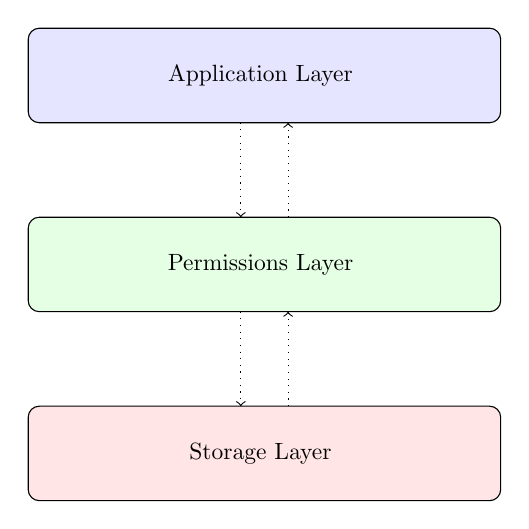
\begin{tikzpicture}[scale = 0.6, every node/.style={scale = 0.85}, every node/.append style={fill = white, rounded corners = 2pt, inner sep = 2pt, align = center}]
  
  % Layer boxes
  \draw [rounded corners, fill=blue!10] (-5, 5) rectangle (5, 3);
  \node [fill=blue!10] at (0, 4) { Application Layer };
  
  \draw [ -> , dotted] (-0.5, 3) -- (-0.5, 1);
  \draw [ -> , dotted] (0.5,  1) -- (0.5,  3);
  
  \draw [rounded corners, fill=green!10] (-5, 1) rectangle (5, -1);
  \node [fill=green!10] at (0, 0) { Permissions Layer };
  
  \draw [ -> , dotted] (-0.5, -1) -- (-0.5, -3);
  \draw [ -> , dotted] (0.5,  -3) -- (0.5,  -1);
  
  \draw [rounded corners, fill=red!10] (-5, -5) rectangle (5, -3);
  \node [fill=red!10] at (0, -4) { Storage Layer };
  
  \end{tikzpicture} \\
  \caption{
  	Platform Layer Communication (Centralised)
  }
  \label{fig:archi_platform_layers_centralised}
\end{figure}

In contrast to the above, a truly decentralised platform communicates such that any one layer can access any other without any intermediaries. This is crucial in stopping any denial of data access, and is one of the core goals of this project.

\begin{figure}[H]
  \centering
  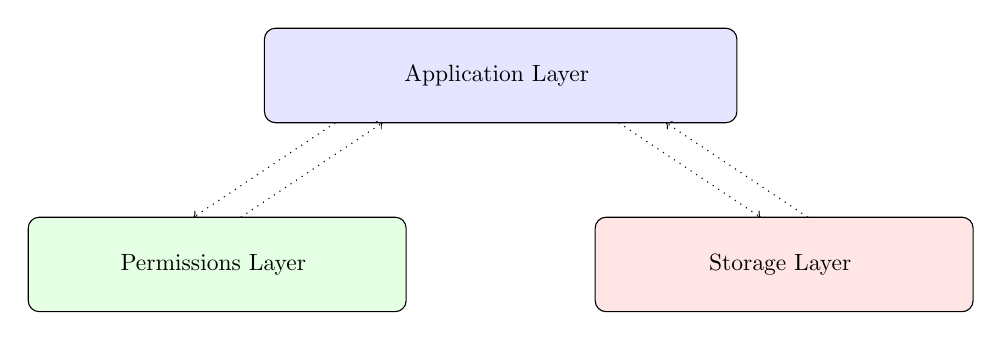
\begin{tikzpicture}[scale = 0.6, every node/.style={scale = 0.85}, every node/.append style={fill = white, rounded corners = 2pt, inner sep = 2pt, align = center}]
  
  % Layer boxes
  \draw [rounded corners, fill=blue!10] (-5, 5) rectangle (5, 3);
  \node [fill=blue!10] at (0, 4) { Application Layer };
  
  \draw [ -> , dotted] (-3.5, 3) -- (-6.5, 1);
  \draw [ -> , dotted] (-5.5,  1) -- (-2.5,  3);
  
  \draw [rounded corners, fill=green!10] (-10, 1) rectangle (-2, -1);
  \node [fill=green!10] at (-6, 0) { Permissions Layer };
  
  \draw [ -> , dotted] (2.5, 3) -- (5.5, 1);
  \draw [ -> , dotted] (6.5,  1) -- (3.5,  3);
  
  \draw [rounded corners, fill=red!10] (2, 1) rectangle (10, -1);
  \node [fill=red!10] at (6, 0) { Storage Layer };
  
  \end{tikzpicture} \\
  \caption{
  	Platform Layer Communication (Decentralised)
  }
  \label{fig:archi_platform_layers_decentralised}
\end{figure}

Whilst figure \ref{fig:archi_platform_layers_decentralised} does not show communication between the permissions layer and storage layer, this is not restricted by the layer architecture but the underlying implementation.
